\scanpage{79}
In the proof, essential use is made of the Hilbert polynomial, in fact we get a solution as a disjoint sum of subschemes of $S$ corresponding to various Hilbert polynomials. Still I would expect that the \deleted{\unsure{solution}} functor is representable as soon as $X/S$ is proper. In view of the application we have in mind here, it would be sufficient (for an\unsure{\deleted{y}|y} integral $S$) to findin $S$ a non empty \deleted{\unsure{set}} open set $S_{\unsure{1|i}}$ such Problem A has always a solution for $X_1=X\mathbin{x}_S S_1$ over $S_1$ . To prove this weeker existence result, it is well possible that a reduction to the projective case is possible, using Chow's lemma and some induction on the relative \unsure{dimension} perhaps. I also would expect that a proof will be easier when working over a complete noetherian local ring, hence the case of a
% The source fragment is drawn once to retain the interlinear word and the hand correction strokes. The baseline word local remains live.
\begin{minipage}[c]{4.7cm}
\figure{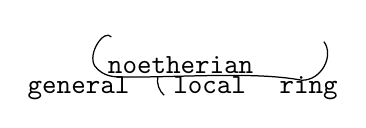
\begin{tikzpicture}[x=1cm,y=1cm]
  \node[anchor=base west,inner sep=0pt,font=\ttfamily] at (0,0) {general};
  \node[anchor=base west,inner sep=0pt,font=\ttfamily] at (1.85,0) {local};
  \node[anchor=base west,inner sep=0pt,font=\ttfamily] at (3.20,0) {ring};
  \node[anchor=base west,inner sep=0pt,font=\ttfamily] at (1.02,0.25) {\inserted{noetherian}};
  \handwritten{
  \draw[line width=0.45pt] (1.07,0.72)
    .. controls (0.98,0.83) and (0.76,0.51) .. (0.86,0.35)
    .. controls (0.97,0.21) and (1.11,0.21) .. (1.25,0.21)
    .. controls (2.04,0.21) and (2.91,0.28) .. (3.49,0.17)
    .. controls (3.74,0.17) and (3.90,0.48) .. (3.77,0.66);
  \draw[line width=0.45pt] (1.66,0.22)
    .. controls (1.64,0.13) and (1.68,0.03) .. (1.74,-0.02);
  }
\end{tikzpicture}}
\end{minipage}
by flat descent. And it is well possible that, putting together two such partial results, a proof of the existence in general could be obtained. (I met with such difficulties allready time ago in a very \unsure{analognous|analoguous} non projective existence problem, which beside I did not solve so far !). This problem A has been met also by Hartshorne (a Harvard student), but I doubt he will work seriously on it. Thus \deleted{to}\handwritten{\unsure{J|I}} now wrote you in the hope you may be interested to have a try on this problem. As a general fact , our knowledge of non projective existence theorems is exceedingly poor, and I hope this will change eventually.

\noindent\hspace*{1cm}Sincerely yours\hfill\handwritten{A Grothendieck}\par
% archive sheet number: 78

